\section{Introdução}

\begin{frame}{Pure Data}
\begin{figure}
\centering
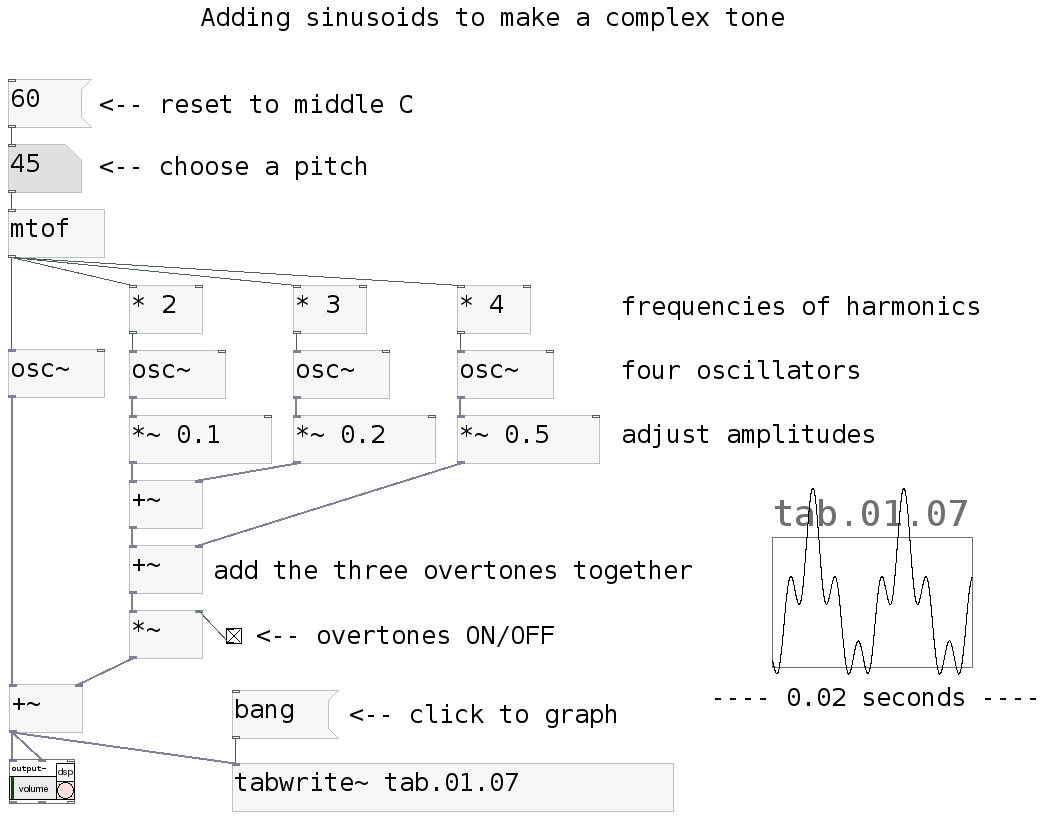
\includegraphics[width=0.7\textwidth]{../images/pd-facil}
\end{figure}
\end{frame}


\begin{frame}{Formas de estender o Pure Data}
Existem algumas formas de estender as funcionalidades do Pure Data:
\begin{itemize}
\item Subpatches.
\item \enfasel{Externals}.
\item Alterações no código-fonte.
\end{itemize}
\pause
\vspace{1em}
Este seminário trata da extensão do Pure Data através da criação de
\externals em C.
\end{frame}


\begin{frame}[fragile]{Organização do código-fonte}
Algumas informações sobre o código do Pure Data:
\begin{itemize}
\item Publicado sob a licença \enfasel{Standard Improved BSD License}.
\item Organizado de forma orientada a objetos.
\begin{itemize}
\item Classes são tipos.
\item Objetos (gráficos) do Pure Data são instâncias de classes.
dados e assinaturas de funções: \texttt{m\_pd.h}.
\end{itemize}
\item Existe um arquivo de cabeçalho com constantes, tipos, estruturas de
dados e assinaturas de funções: \texttt{m\_pd.h}.
\end{itemize}
\end{frame}


\begin{frame}[fragile]{Compilação}
\begin{lstlisting}
EXTNAME=meu_external
cc -DPD -fPIC -Wall -o ${EXTNAME}.o -c ${EXTNAME}.c
ld -shared -lc -lm -o ${EXTNAME}.pd_linux ${EXTNAME}.o
rm ${EXTNAME}.o
\end{lstlisting}
O Pure Data procura por objetos com nomes diferentes em cada sistema:
\begin{itemize}
  \item \texttt{meu\_external.\enfase{pd\_linux}} (GNU/Linux).
  \item \texttt{meu\_external.\enfase{pd\_irix5}} (Irix 5).
  \item \texttt{meu\_external.\enfase{pd\_darwin}} (Mac OS X).
  \item \texttt{meu\_external.\enfase{dll}} (MS Windows).
\end{itemize}
\end{frame}


\begin{frame}[fragile]{Arquivos de ajuda}
Um arquivo de ajuda é um patch do Pure Data com:
\begin{itemize}
\item Um nome informativo: \texttt{meu\_external\enfase{-help}.pd}.
\item Instruções de uso.
\item Exemplos de utilização.
\end{itemize}
\vspace{2em}
A seguinte função associa um arquivo de ajuda a uma classe de \external:
\begin{lstlisting}
class_sethelpsymbol(meu_external_class, gensym("meu_external_class-help"));
\end{lstlisting}
\end{frame}


\begin{frame}{Utilizando \externals}
Passos para utilizar um \external no Pure Data:
\begin{enumerate}
\item Escreva um arquivo \texttt{.c} com as funções, classes e métodos.
\item Compile o código-fonte para criar uma biblioteca compartilhada.
\item Informe ao Pure Data o caminho para o \external através de uma das
opções abaixo:
  \begin{itemize}
    \item Na criação do objeto, insira o caminho completo (relativo ou
    absoluto) para o objeto do \external.
    \item Na linha de comando, utilize a opção \enfasel{\texttt{-path
    <caminho>}}.
    \item Na interface gráfica, acesse a opção \enfasel{\texttt{File} $\rightarrow$
    \texttt{Path...}}.
  \end{itemize}
\item Crie um objeto na interface gráfica do Pd com o nome do arquivo do \external, sem a extensão.
\end{enumerate}
\end{frame}


\begin{frame}{Utilizando \externals}
\begin{figure}[h!]
  \centering
  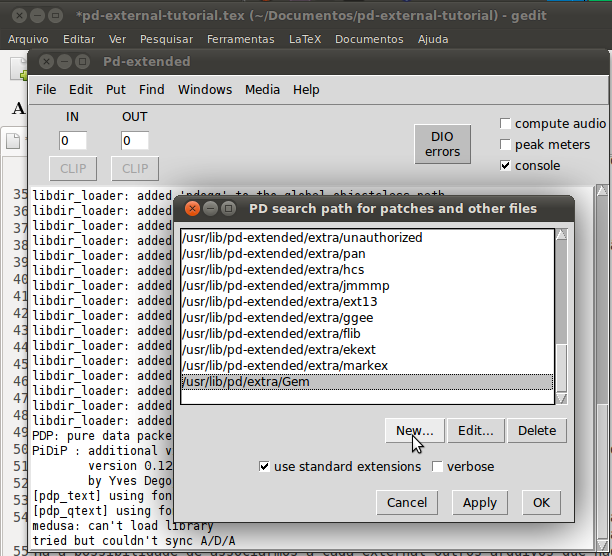
\includegraphics[width=0.7\textwidth]{../images/path}
  \caption{Adicionando o diretório de um \external ao caminho de busca do Pure Data.}
  \label{fig:search-path}
\end{figure}
\begin{itemize}
\item
\end{itemize}
\end{frame}
